\documentclass[12pt]{article}%
\usepackage{amsfonts}
\usepackage{fancyhdr}
\usepackage{comment}
\usepackage[letterpaper, top=2.5cm, bottom=2.5cm, left=2.2cm, right=2.2cm]%
{geometry}
\usepackage{times}
\usepackage{amsmath}
\usepackage{changepage}
\usepackage{multirow}
\usepackage{amssymb}
\usepackage{graphicx}%
\graphicspath{ {images/} }
\usepackage{amsmath}
\setcounter{MaxMatrixCols}{30}
\newtheorem{theorem}{Theorem}
\newtheorem{acknowledgement}[theorem]{Acknowledgement}
\newtheorem{algorithm}[theorem]{Algorithm}
\newtheorem{axiom}{Axiom}
\newtheorem{case}[theorem]{Case}
\newtheorem{claim}[theorem]{Claim}
\newtheorem{conclusion}[theorem]{Conclusion}
\newtheorem{condition}[theorem]{Condition}
\newtheorem{conjecture}[theorem]{Conjecture}
\newtheorem{corollary}[theorem]{Corollary}
\newtheorem{criterion}[theorem]{Criterion}
\newtheorem{definition}[theorem]{Definition}
\newtheorem{example}[theorem]{Example}
\newtheorem{exercise}[theorem]{Exercise}
\newtheorem{lemma}[theorem]{Lemma}
\newtheorem{notation}[theorem]{Notation}
\newtheorem{problem}[theorem]{Problem}
\newtheorem{proposition}[theorem]{Proposition}
\newtheorem{remark}[theorem]{Remark}
\newtheorem{solution}[theorem]{Solution}
\newtheorem{summary}[theorem]{Summary}
\newenvironment{proof}[1][Proof]{\textbf{#1.} }{\ \rule{0.5em}{0.5em}}

\newcommand{\Q}{\mathbb{Q}}
\newcommand{\R}{\mathbb{R}}
\newcommand{\C}{\mathbb{C}}
\newcommand{\Z}{\mathbb{Z}}

\newcommand*{\pd}[3][]{\ensuremath{\frac{\partial^{#1} #2}{\partial #3}}}

\usepackage{enumerate}% http://ctan.org/pkg/enumerate
\usepackage{array}% http://ctan.org/pkg/array
\newcolumntype{M}{>{$}c<{$}}


\begin{document}

\title{CS 440/ECE448 Homework 1}
\author{Tanishq Dubey (tdubey3)}
\date{\today}
\maketitle
\section*{Problem 1}
\begin{enumerate}[(a)]
  \item
  \begin{enumerate}[i.]
  \item
        DFS
        \newline
        \begin{center}
        \hfill\begin{tabular}{c | c} % centered columns (s columns)
            \hline\hline %inserts double horizontal lines
            Node & Stack \\ [0.5ex] % inserts table
            %heading
            \hline % inserts single horizontal line
            - & \{A\}  \\ % inserting body of the table
            A & \{B C D\}  \\
            B & \{E F C D\}  \\
            E & \{J F C D\}  \\ 
            J & \{F C D\}  \\ [1ex] % [1ex] adds vertical space
            \hline %inserts single line
        \end{tabular}\hfill\null
        \end{center}
        \begin{center}
            \textit{Goal Found: J}
        \end{center}
    \item
        BFS
        \newline
        \begin{center}
        \hfill\begin{tabular}{c | c} % centered columns (s columns)
            \hline\hline %inserts double horizontal lines
            Node & Queue \\ [0.5ex] % inserts table
            %heading
            \hline % inserts single horizontal line
            - & \{A\}  \\ % inserting body of the table
            A & \{B C D\}  \\
            B & \{C D E F\}  \\
            C & \{D E F G H\}  \\
            D & \{E F G H I\}  \\
            E & \{F G H I J\}  \\
            F & \{G H I J\}  \\
            G & \{H I J K L\}  \\ 
            H & \{I J K L\}  \\  [1ex] % [1ex] adds vertical space
            \hline %inserts single line
        \end{tabular}\hfill\null
        \end{center}
        \begin{center}
            \textit{Goal Found: H}
        \end{center}
    \break
    \item
        Greedy
        \newline
        \begin{center}
        \hfill\begin{tabular}{c | c} % centered columns (s columns)
            \hline\hline %inserts double horizontal lines
            Node & Queue \\ [0.5ex] % inserts table
            %heading
            \hline % inserts single horizontal line
            - & \{A\}  \\ % inserting body of the table
            A & \{C B D\}  \\
            C & \{H D B G\}  \\ 
            H & \{D B G \}  \\ [1ex] % [1ex] adds vertical space
            \hline %inserts single line
        \end{tabular}\hfill\null
        \end{center}
        \begin{center}
            \textit{Goal Found: H}
        \end{center}
    \item
        Uniform Cost
        \newline
        \begin{center}
        \hfill\begin{tabular}{c | c} % centered columns (s columns)
            \hline\hline %inserts double horizontal lines
            Node & Queue \\ [0.5ex] % inserts table
            %heading
            \hline % inserts single horizontal line
            - & \{A\}  \\ % inserting body of the table
            A & \{C D B\}  \\
            C & \{D B G H\}  \\
            D & \{B G I H\}  \\
            B & \{E G F I H\}  \\
            E & \{G F I H J\}  \\
            G & \{F I H K J K L\}  \\
            F & \{I H K J K L\}  \\
            I & \{H K J K L\}  \\ [1ex] % [1ex] adds vertical space
            \hline %inserts single line
        \end{tabular}\hfill\null
        \end{center}
        \begin{center}
            \textit{Goal Found: I}
        \end{center}
    \item
        A*
        \newline
        \begin{center}
        \hfill\begin{tabular}{c | c} % centered columns (s columns)
            \hline\hline %inserts double horizontal lines
            Node & Queue \\ [0.5ex] % inserts table
            %heading
            \hline % inserts single horizontal line
            - & \{A\}  \\ % inserting body of the table
            A & \{C D B\}  \\
            C & \{D B G H\}  \\
            D & \{I B G H\}  \\
            I & \{ B G H\}  \\ [1ex] % [1ex] adds vertical space
            \hline %inserts single line
        \end{tabular}\hfill\null
        \newline
        \end{center}
        \begin{center}
            \textit{Goal Found: I}
        \end{center}
  \end{enumerate}
  \item
  In this example, the heuristic \textit{h} is both admissible and consistent. The heuristic is admissible because \textit{h} never over estimates the cost to the goal. For example, looking at the path from \textit{A}$\,\to\,$\textit{I} we can see that the heuristic cost is never greater than the path cost. In fact this is true for every path, and so the heuristic is admissible. In addition, the heuristic is consistent. This can be proven through the observation that the sum of the current node and the next node does not exceed the cost of the path between the nodes. Due to this, the heuristic is admissible.
  \newline
  \item
  \break
  \begin{enumerate}[i.]
    \item DFS will not always find the best solution, instead DFS will return the first solution it sees.
    \item BFS will not always find the best solution, instead BFS will return the first solution it sees.
    \item Greedy search will not always find the best solution, this is because greedy will pick the path of the shortest path, ignoring the heuristic.
    \item Uniform search will always find the best solution. This occurs because uniform search essentially ignores the path weight and instead uses the heuristic to find a solution.
    \item A* search will only always find the best solution when the heuristic is admissible.
  \end{enumerate}
\end{enumerate}

\section*{Problem 2}
    \begin{enumerate}[(a)]
        \item The partial derivatives of:
            \[ f(x,y) = a_1x^2 + a_2y^2 + b_1xy + c_1x + c_2y\]
            are:
            \[\pd{f}{x} = 2a_1x + b_1y + c_1 \]
            and
            \[\pd{f}{y} = 2a_2y + b_1x + c_2 \]
        \item
            Given that \[ a_1 = a_2 = b_1 = c_1 = c_2 = 1 \]
            The convexity, or lack thereof, of the function $f(x,y)$ over the feasible region $[0,1]^2$ can be proven using the Hessian matrix of the function, which is:
            \newline
            \begin{center}
             H =
                \begin{bmatrix}
                    \pd{^2f}{x^2} & \pd{^2f}{x\partial y} \\
                    \pd{^2f}{y\partial x} & \pd{^2f}{y^2}  \\
                \end{bmatrix}
            \end{center}
            We can then substitute in our values for the second order partial derivatives to get:
            \begin{center}
             H =
                \begin{bmatrix}
                    2a_1 & b_1 \\
                    b_1 & 2a_2 \\
                \end{bmatrix}
            \end{center}
            And with our previously given values for $a_1, a_2, b_1,$ and $b_2$, we substitute to get:
            \begin{center}
             H =
                \begin{bmatrix}
                    2 & 1 \\
                    1 & 2 \\
                \end{bmatrix}
            \end{center}
            By determining if the matrix $H$ is a positive definite matrix, or more generally, by determining that $z^TMz$ is positive for every non-zero column vector $z$ of $n$ real numbers where $z^T$ represents the transpose of $z$ and $M$ is our matrix. Thus if we consider: $v =$
            \begin{bmatrix}
                a \\
                b \\
            \end{bmatrix}
            we can find the transpose of $v$ with $H$, which results in $a^2 + ab + b^2$. Now we must assume that this transpose positive, thus:
                \[ a^2 + ab + b^2 > 0\]
                \break
            To ensure that this assumption is true, proving that the matrix is positive definite, a number of cases must be examined:
            \begin{enumerate}[1. ]
                \item If both $a$ and $b$ are positive then the transpose evaluates to positive
                \item If both $a$ and $b$ are negative, then the transpose also evaluates to positive. The case of the transpose evaluating to 0 is avoided because $a$ and $b$ cannot both be 0.
                \item If $a$ and $b$ are opposite signs, the transpose evaluates to positive.
                \item If $a$ is 0, then the transpose is positive because b cannot be 0.
                \item if $b$ is 0, then the transpose is positive because a cannot be 0.
            \end{enumerate}
            Since it is shown that in all cases of $(a,b)$ the transpose matrix is positive, it can be said that the matrix $H$ is a positive definite matrix, which implies that the matrix is also positive semidefinite. A result of this implication is that the function of a positive semidefinite matrix is also convex. Thus, it is shown that $f(x,y)$ is convex.
        \item
            Given that \[ a_1 = a_2 = 1 b_1 = 5 c_1 = c_2 = 3 \]
            The convexity, or lack thereof, of the function $f(x,y)$ over the feasible region $[-1,1]^2$ can be proven using the Hessian matrix of the function, which is:
            \newline
            \begin{center}
             H =
                \begin{bmatrix}
                    \pd{^2f}{x^2} & \pd{^2f}{x\partial y} \\
                    \pd{^2f}{y\partial x} & \pd{^2f}{y^2}  \\
                \end{bmatrix}
            \end{center}
            We can then substitute in our values for the second order partial derivatives to get:
            \begin{center}
             H =
                \begin{bmatrix}
                    2a_1 & b_1 \\
                    b_1 & 2a_2 \\
                \end{bmatrix}
            \end{center}
            And with our previously given values for $a_1, a_2, b_1,$ and $b_2$, we substitute to get:
            \begin{center}
             H =
                \begin{bmatrix}
                    2 & 5 \\
                    5 & 2 \\
                \end{bmatrix}
            \end{center}
            It can be clearly seen that the procedure of finding if the matrix $H$ is a positive definite matrix outlined above is sufficient in determining the convexity of the given function. So, the transpose function is once again found:
                \[ a^2 + 5ab + b^2 > 0\]
            Then similar test cases are proven or disproven to find convexity.
            \begin{enumerate}[1. ]
                \item If both $a$ and $b$ are positive then the transpose evaluates to positive
                \item If both $a$ and $b$ are negative, then the transpose also evaluates to positive. The case of the transpose evaluating to 0 is avoided because $a$ and $b$ cannot both be 0.
                \item If $a$ and $b$ are opposite signs, then the transpose does not evaluate to be positive.
                \item If $a$ is 0, then the transpose is positive because b cannot be 0.
                \item if $b$ is 0, then the transpose is positive because a cannot be 0.
            \end{enumerate}
            Since it is shown that the third test case breaks our assumption of finding a positive definite matrix, it cannot be said that the function $f(x,y)$ is convex. Instead graphing software can be used to determine that with the given constants, the function has a saddle point in the given feasible region.
            \begin{center}
                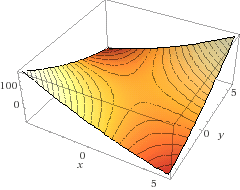
\includegraphics[scale=.75]{graph}
            \end{center}
    \end{enumerate}
\end{document}